%% --------------------------------------------------------------
%%
%% I N T R O D U C T I O N
%%
%% --------------------------------------------------------------

\begin{frame}%{Binary neutron star (BNS) mergers}  %% ---------- Intro/motivation 

\begin{tikzpicture}[overlay,remember picture]

\uncover<1->{ % <-> |
    \node (t1) [anchor=center,scale=1,opacity=1] at ([shift={(-4.0cm,3.0cm)}]current page.center){
        \parbox{0.5\textwidth}{
        \begin{footnotesize}
            \textbf{Neutron stars (NSs)} are cores of massive stars, after core collapse supernovae.
            % which had a total mass of between 10 and 25 solar masses
%            Unknown inner structure \\
%            If in binary, they will collide \\ 
        \end{footnotesize}
    }};
}
\uncover<1->{ % <-> |
    \node (t1) [anchor=center,scale=1,opacity=1] at ([shift={(-4.0cm,0.0cm)}]current page.center){
        \parbox{0.55\textwidth}{
            \textit{Binary neutron star (BNS) mergers} relate to
            \begin{itemize}
                \item origin of heaviest elements;
                \item origin of kilonovae and (some) short \acp{GRB};
                \item theory of gravity;
                \item cosmology;
                %\item \nuc{} of the heaviest elements in the Universe,
                %\item cosmology.%, using \ac{BNS} mergers as standard sirens
            \end{itemize}
    }};
}
\uncover<1->{ % <-> |
    \node (t1) [anchor=center,scale=1,opacity=1] at ([shift={(-4.0cm,-3.0cm)}]current page.center){
        \parbox{0.55\textwidth}{
            \textit{Numerical relativity (NR) simulations} $\rightarrow$ 
            % \vspace{-5mm}
            \begin{itemize}
                \item \acp{GW};
                \item ejecta properties.
            \end{itemize}
    }};
}
\uncover<1->{ % <-> |
    \node (img1) [anchor=center,scale=1,opacity=1] at ([shift={(3.4cm,-0.2cm)}]current page.center){
        \parbox{0.5\textwidth}{
            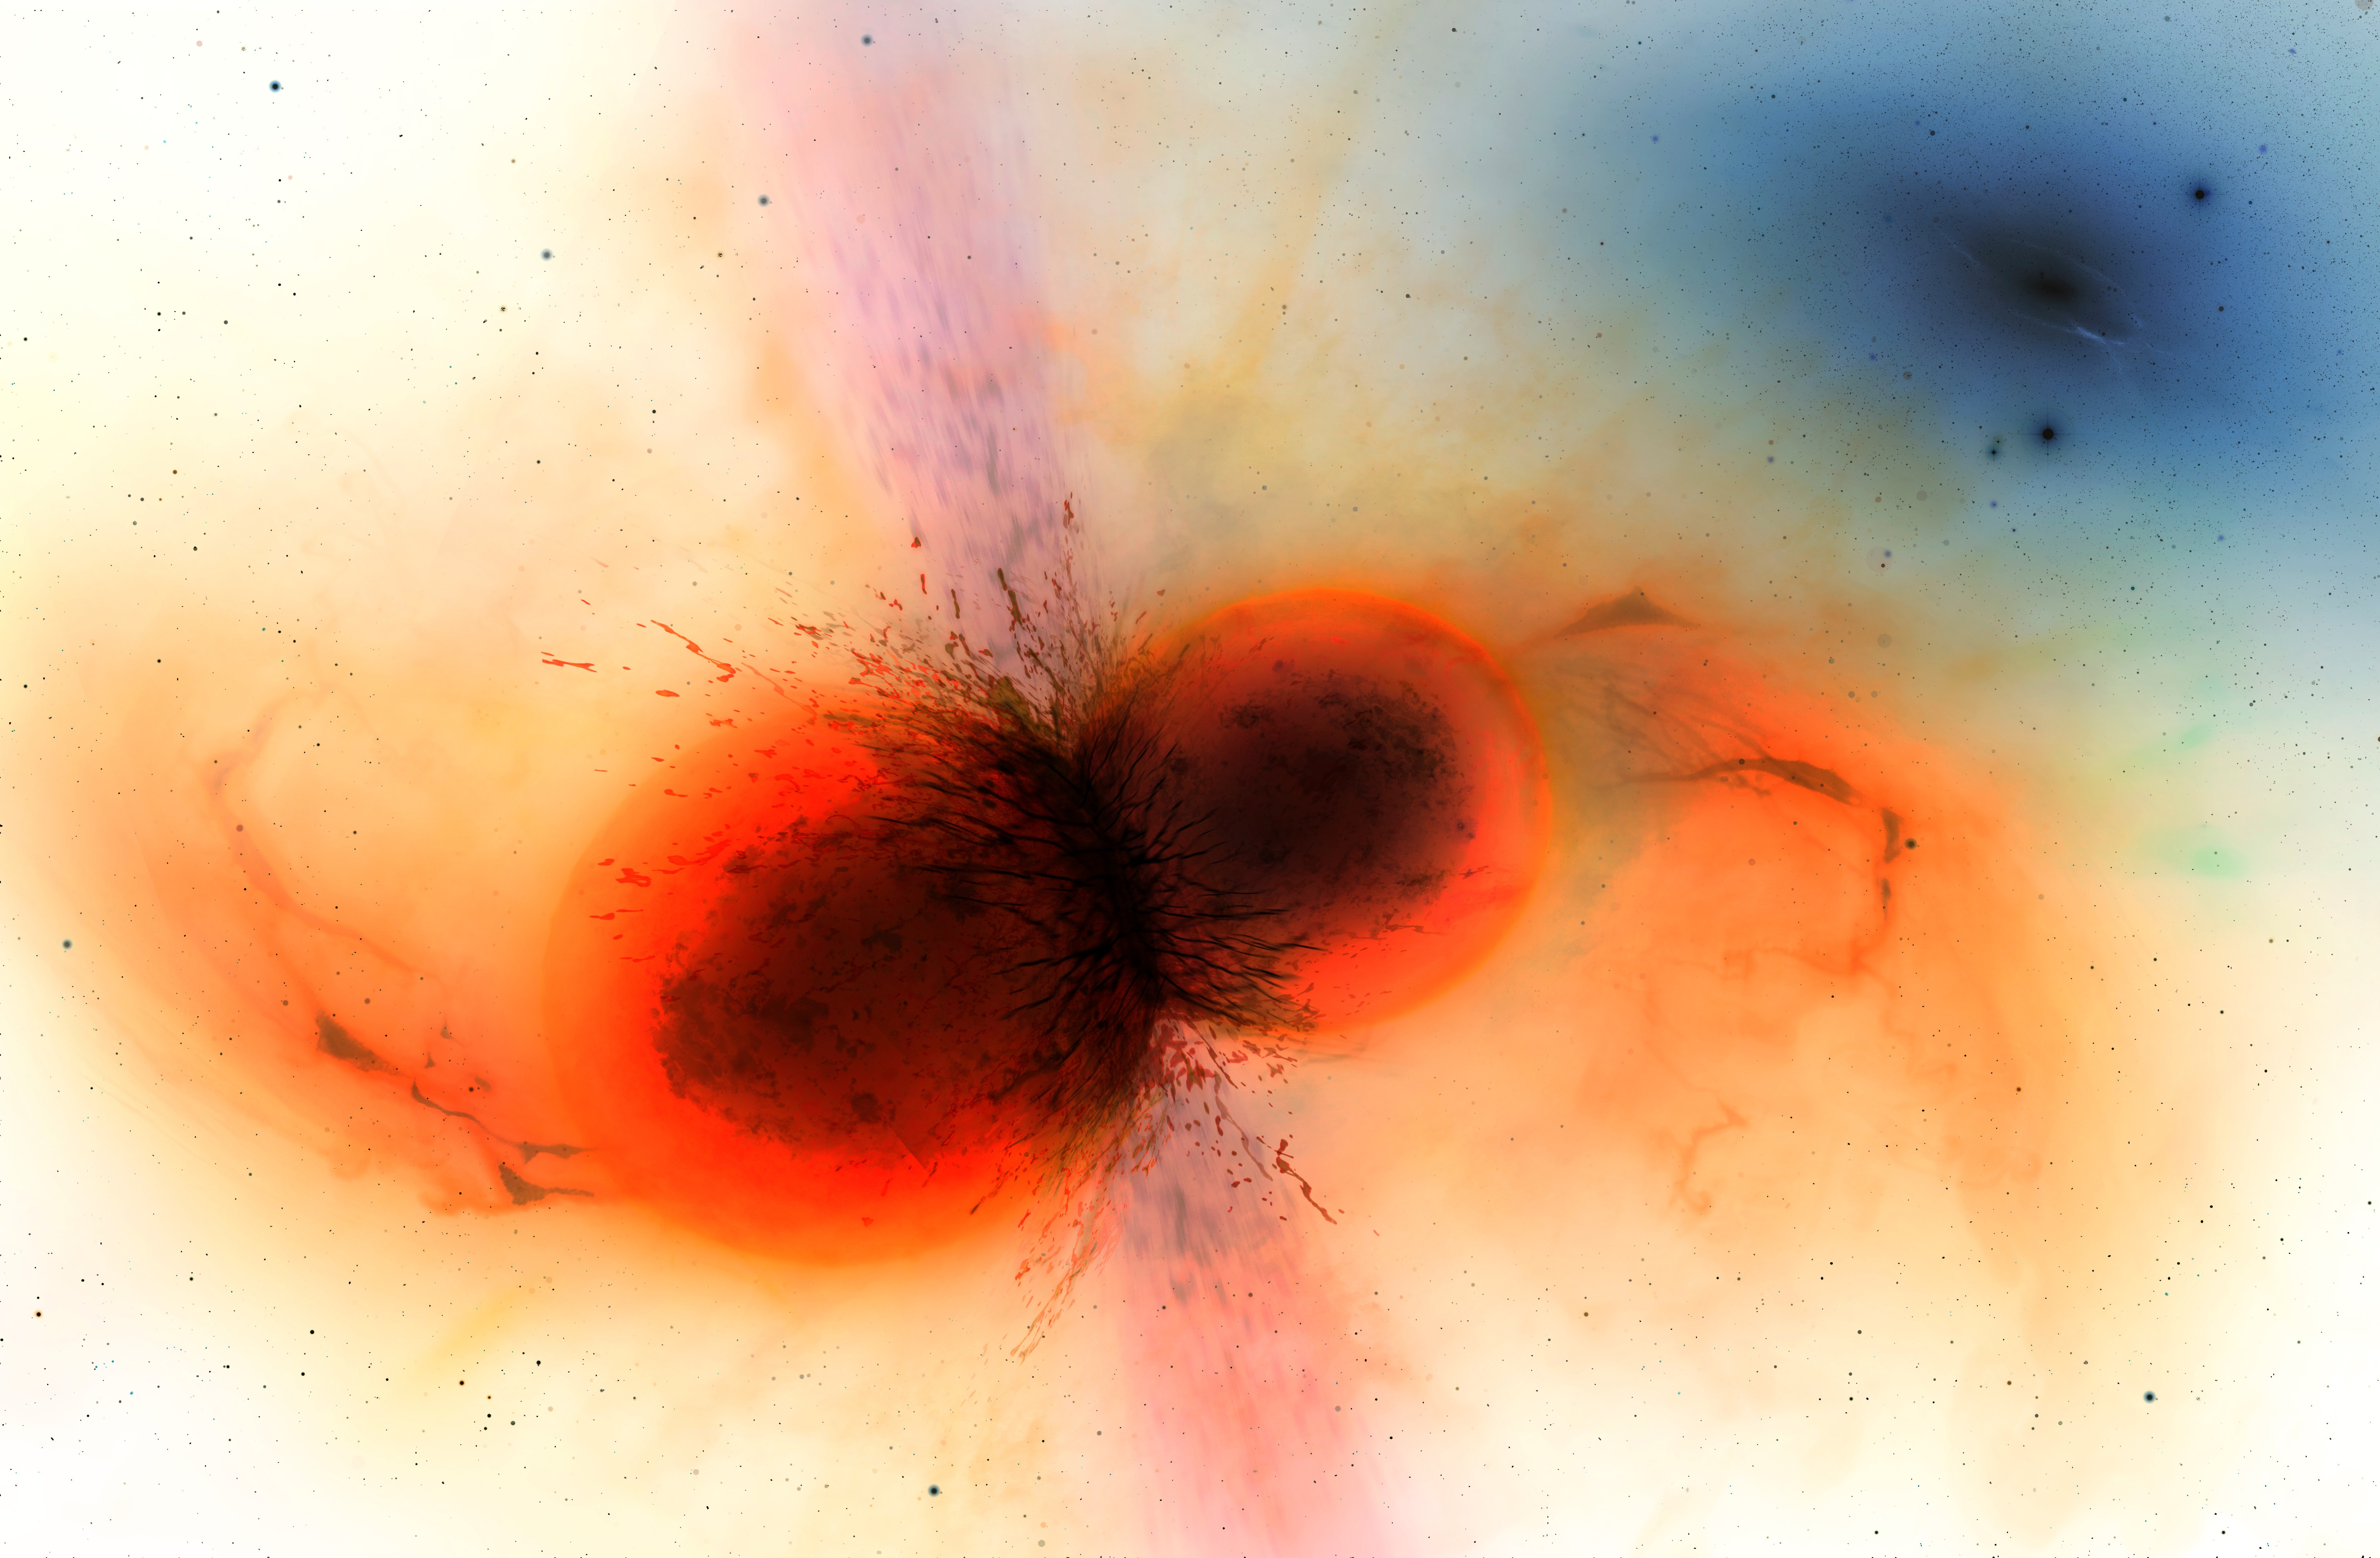
\includegraphics[height=5.3cm]{figures/bns_cartoon_inveted.jpg}\\
            Artist depiction of merging neutron stars. \\
            \textcolor{gray}{ \footnotesize{
                    Credit: University of Warwick/Mark Garlick} 
                }
    }};
}


\end{tikzpicture}
\end{frame}

%% ----------------------------------------------------------------------------------

\begin{frame}%{Binary neutron star (BNS) mergers}  %% ---------- Intro/motivation 
    
    \begin{tikzpicture}[overlay,remember picture]
        \uncover<1->{ % <-> |
            \node (t1) [anchor=center,scale=1,opacity=1] at ([shift={(-3.6cm,2.0cm)}]current page.center){
                \parbox{0.60\textwidth}{
                    August 2017, \textbf{multimessenger event}: 
                    \begin{itemize}
                        \item \GW{} -- \ac{GW};
                        \item \AT{} -- thermal \ac{EM} emission, kilonova; %thermal electromagnetic (EM) emission, kilonova (kN), \AT{},
                        \item \GRB{} -- non-thermal \ac{EM} short \ac{GRB}.% non-thermal \ac{EM} short gamma-ray burst (GRB), \GRB{}
                    \end{itemize}
                    
                    %            Wealth of information about different physical processes occurring in BNS\\
                    %\red{Questions}: remnant's lifetime; ejecta mass/composition; sources of \rproc{} elements
            }};
        }
        
        \uncover<1->{ % <-> |
            \node (t1) [anchor=center,scale=1,opacity=1] at ([shift={(-3.6cm,0.0cm)}]current page.center){
                \parbox{0.60\textwidth}{
                     \textit{\ac{EM} models} $\rightarrow$ ejecta properties.
            }};
        }
    
        \uncover<1->{ % <-> |
            \node (t1) [anchor=center,scale=1,opacity=1] at ([shift={(-3.6cm,-2.0cm)}]current page.center){
                \parbox{0.60\textwidth}{
                    What are the parameters and 
                    what is the \ac{NS} \textbf{\ac{EOS}}?
                    %by using \ac{NR} simulations and \ac{EM} counterparts 
            }};
        }
    
%        \uncover<1->{ % <-> |
%            \node (t1) [anchor=center,scale=1,opacity=1] at ([shift={(0.0cm,-3.4cm)}]current page.center){                    Artist depiction of merging neutron stars \\
%                \textcolor{gray}{ \footnotesize{
%                        Credit: University of Warwick/Mark Garlick} 
%                }
%                \parbox{1.1\textwidth}{
%                    %            \textcolor{black}{Major advanclemts} were maid in our understanding of related physical processes \\
%                    \textcolor{black}{ \textbf{Key questions}}: remnant fate; origin of the early kilonova emission; origin of the late \ac{GRB} afterglow; \\
%                    \textbf{What is NS equation of state (\ac{EOS})?}
%            }};
%        }
        
        \uncover<1->{ % <-> |
            \node (img1) [anchor=center,scale=1,opacity=1] at ([shift={(4.7cm,0.1cm)}]current page.center){
                \parbox{0.4\textwidth}{
                    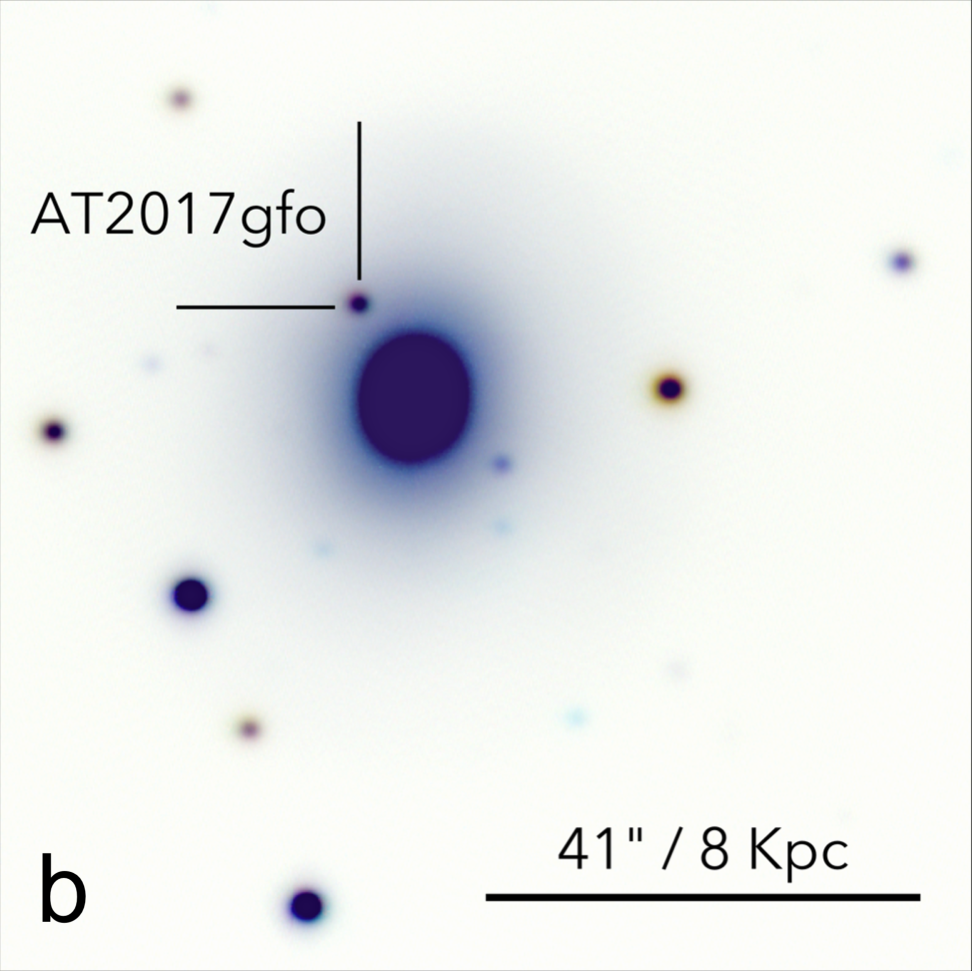
\includegraphics[height=5.8cm]{figures/at2017gfo_smartt_inv.png}\\
                    Image of AT2017gfo\footcite{Smartt:2017fuw}
                    %$^{\textcolor{gray}{\text{\cite{Smartt:2017fuw}}}}$
            }};
        }
        
    \end{tikzpicture}
\end{frame}